\documentclass{article}
\usepackage[utf8]{inputenc}
\usepackage[letterpaper, portrait, margin=1in]{geometry}
\usepackage{enumerate}
% Display only levels as deep as subsection in tableofcontents
\setcounter{tocdepth}{2}

\usepackage{caption}
\usepackage{graphicx}
\graphicspath{ {images/} }
\usepackage{array}

\usepackage{multirow,booktabs}

% Define function subcommands
\newcommand{\name}[1]{\hline \multicolumn{2}{|l|}{\texttt{#1}} }
\newcommand{\inp}[1]{\hline \textbf{Input:} & #1}
\newcommand{\out}[1]{\hline \textbf{Output:} & #1}
\newcommand{\desc}[1]{\hline \textbf{Description:} & #1 }

% Define function command
\newcommand{\fcn}[4]{
    \begin{center}
    \begin{tabular}{|p{2cm} p{10cm}|}
    \hline
    \name{#1} \\
    \inp{#2} \\
    \out{#3} \\
    \desc{#4} \\
    \hline
    \end{tabular}
    \end{center}
}

%%%%%%%%%%%%%%%%%%%%%%%%%%%%%%%%%%%%%%%%%%%%%%%%%%%%%%%%%%%%%%%%%%%%%%%%%%%%%
% GRAPHS
%%%%%%%%%%%%%%%%%%%%%%%%%%%%%%%%%%%%%%%%%%%%%%%%%%%%%%%%%%%%%%%%%%%%%%%%%%%%%
\usepackage{tikz}
\usepackage{verbatim}
\usetikzlibrary{positioning,arrows,shapes}
%%%%%%%%%%%%%%%%%%%%%%%%%%%%%%%%%%%%%%%%%%%%%%%%%%%
% HEADER
%%%%%%%%%%%%%%%%%%%%%%%%%%%%%%%%%%%%%%%%%%%%%%%%%%%
\usepackage{fancyhdr}
\pagestyle{fancy}
\fancyhf{}
\fancyhead[C]{PiSonal Trainer: Weight Lifting Performance Tracker}
\fancyfoot[L]{System Architecture}
\fancyfoot[R]{\thepage}
\renewcommand{\headrulewidth}{0.4pt}
\renewcommand{\footrulewidth}{0.4pt}

% Use this to pad tables
\usepackage{array}
\setlength\extrarowheight{6pt}

% Define tab command
\newcommand\tab{\hspace*{2cm}}


%%%%%%%%%%%%%%%%%%%%%%%%%%%%%%%%%%%%%%%%%%%%%%%%%%%
% TITLE
%%%%%%%%%%%%%%%%%%%%%%%%%%%%%%%%%%%%%%%%%%%%%%%%%%%
\title{
PiSonal Trainer: Weight Lifting Performance Tracker\\
\Large {System Architecture}
}
\date{April 1, 2017}
\author{Birunthaa Umamahesan \and Micaela Estabillo \and Simarpreet Singh}

\begin{document}
%%%%%%%%%%%%%%%%%%%%%%%%%%%%%%%%%%%%%%%%%%%%%%%%%%%
% COVER PAGE
%%%%%%%%%%%%%%%%%%%%%%%%%%%%%%%%%%%%%%%%%%%%%%%%%%%
\thispagestyle{plain}
\pagenumbering{gobble}
\maketitle
\vfill
\begin{center}
    Prepared for Computer Science 4ZP6: Capstone Project \\
    Instructor: Dr. Wenbo He
    Fall/Winter 2016-2017\\
\end{center}
\newpage

%%%%%%%%%%%%%%%%%%%%%%%%%%%%%%%%%%%%%%%%%%%%%%%%%%%
% TABLE OF CONTENTS AND REVISION HISTORY
%%%%%%%%%%%%%%%%%%%%%%%%%%%%%%%%%%%%%%%%%%%%%%%%%%%
\tableofcontents

\listoffigures

\listoftables

\thispagestyle{plain}
\pagenumbering{gobble}

\newpage

\section*{Revision History}
\begingroup
\begin{tabular}{ | p{2cm} | p{1.5cm} | p{3.8cm} | p{7cm} |} 
    \hline
    \textbf{Date} & \textbf{Version} & \textbf{Primary Author} & \textbf{Comment}\\
    \hline
    4/1/2017 & 1.00 & Birunthaa Umamahesan & Proofread document for revision 1\\ 
    \hline
    4/1/2017 & 1.00 & Micaela Estabillo & Adjust technical specifications based on changes\\ 
    \hline
    1/11/2017 & 0.00 & Birunthaa Umamahesan & Proofread document for revision 0\\
    \hline
    1/11/2017 & 0.00 & Micaela Estabillo & Finalize document draft\\
    \hline
    1/9/2017 & 0.00 & Micaela Estabillo & Create document outline\\
    \hline
\end{tabular}
    \captionof{table}{Revision history}
\endgroup


\begin{center}
% Volere Edition 16
%We acknowledge that this document uses material from the Volere Requirements Specification Template, copyright © 1995 – 2012 the Atlantic Systems Guild Limited.
\end{center}

\newpage

\clearpage
\setcounter{page}{1}
\pagenumbering{arabic}

%%%%%%%%%%%%%%%%%%%%%%%%%%%%%%%%%%%%%%%%%%%%%%%%%%%
% 
%%%%%%%%%%%%%%%%%%%%%%%%%%%%%%%%%%%%%%%%%%%%%%%%%%%

\section{Introduction and Overview}
This document provides a description of how PiSonal Trainer will be built. The following are covered in this document:
\begin{itemize}
    %\item An explanation of the templates, symbols and conventions used in the document
    \item Diagram and individual descriptions of the overall component decomposition of the system
    \item Anticipated and unlikely design changes
    \item The Requirements and Design Traceability Matrix relating the system’s components to the project requirements established in the Software Requirements Specifications (SRS) document
\end{itemize}

\section{Decomposition into Components}
The system is decomposed based on its different elements in order to allow each component to be implemented and developed independently. Nevertheless, each component interacts with at least one other.
\begin{enumerate}
\item \textbf{User Interface (UI)}: The UI encompasses the frontend and backend of the mobile app used to track workouts and display performance history. The app communicates with the database containing a collection of authorized users to authenticate. It also sends exercise performance statistics to the database. A mobile platform is ideal for PiSonal Trainer so that users can easily bring their device to their gyms, and record or view their performance.

\item \textbf{Camera and Counting Algorithm}: Since the camera in use is connected to the device itself, the movement counting algorithm is implemented there as well using OpenCV. This is done to reduce resource overhead that would be generated by sending image information for processing to a remote server. The algorithm is discussed in detail in the Detailed Design document.

\item \textbf{Database}: The database keeps unauthorized users from using the app and stores counts pertaining to a user's exercises. User performance graphs are dynamically generated by querying the database and sending data back to the user's phone. All the counts are stored in the database in order to avoid taking up too much space in the phone's disk.
\end{enumerate}



\begingroup
\begin{center}
\begin{figure}[h]
\center{
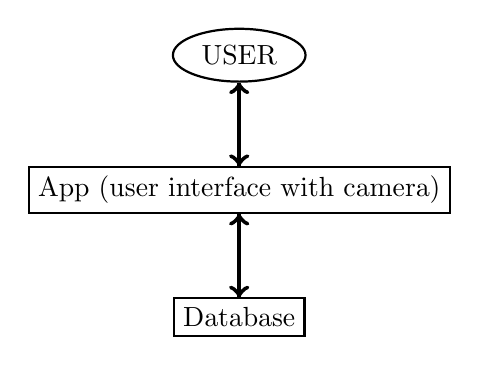
\begin{tikzpicture} [node distance=30pt]
    \node[draw,thick,ellipse] (user) {USER};
    \node[draw,thick,rectangle,below=of user] (ui) {App (user interface with camera)};
    \node[draw,thick,rectangle,below=of ui] (db) {Database};

    \path (user) edge [->,ultra thick] (ui);
    \path (ui) edge [->,ultra thick] (user);
    \path (ui) edge [->,ultra thick] (db);
    \path (db) edge [->,ultra thick] (ui);
\end{tikzpicture}
}
\end{figure}
\end{center}
\captionof{figure}{Interaction of PiSonal Trainer Components}
\endgroup

\newpage
\section{Requirements and Design Traceability Matrix}
The following table contains the functional requirements identified in PiSonal Trainer's Software Requirement Specification document, their descriptions and their corresponding design component/s.
\begingroup
\begin{center}
\begin{tabular}{| p{2.5cm} | p{7cm} | p{3.5cm} |}
    \hline
    \textbf{Requirement} & \textbf{Description} & \textbf{Design Reference} \\
    \hline
    R1 & Only registered users may be able to use the app & UI, Database\\
    R2 & The app shall provide meaningful error messages & UI \\
    R3 & The app shall display the user’s progress statistics through visual graphs & UI, Database \\
    R4 & A camera shall track the motion of the gym equipment & Camera\\
    R5 & The user’s exercise performance data shall be stored for future retrieval & Database \\
    R6 & The user’s performance shall be calculated using data from the camera and the equipment’s weight & UI, Database, Camera \\
    \hline
\end{tabular}
\end{center}
\captionof{table}{Requirements and Design Traceability}
\endgroup


%%%%%%%%%%%%%%%%%%%%%%%%%%%%%%%%%%%%%%%%%%%%%%%%%%%
% REFERENCES
%%%%%%%%%%%%%%%%%%%%%%%%%%%%%%%%%%%%%%%%%%%%%%%%%%%
% \section*{References}

%%%%%%%%%%%%%%%%%%%%%%%%%%%%%%%%%%%%%%%%%%%%%%%%%%%
% INDEX
%%%%%%%%%%%%%%%%%%%%%%%%%%%%%%%%%%%%%%%%%%%%%%%%%%%
%\section*{Index}

\end{document}

The document should include the system architecture design and component design. You should give the architecture of the system, system components, APIs, algorithms used, solutions to address the challenges mentioned in your previous report, and shows the reasons on your design choices.